% !TEX root = /media/ueslei/Ueslei/INPE/PCI/Projetos/Guia_COAWST/main.tex
\chapterimage{ocean2.jpg} % Chapter heading image

\chapter{O COAWST no cluster Kerana}\index{COAWST na Kerana}
\bigskip

\section{Sobre o Kerana}
\bigskip

\noindent A máquina CRAY XE, também chamada de Kerana, é um cluster com arquitetura massivamente paralela,
contando com 84 nós de processamento e 2688 cores e está localizada nas dependências do CPTEC/INPE,
em Cachoeira Paulista, São Paulo. Por contar com a habilidade de paralelizar operações através da interface
Message Passing Interface (MPI), o cluster é ideal para usar modelos numéricos com alta resolução espacial
e temporal.
\bigskip

\section{Registrando uma conta de usuário}
\bigskip

\noindent Para iniciar o processo de requerimento de uma conta de usuário no Kerana, é necessário que o computador nas dependências do INPE possuia IP fixo. É requerido do seu orientador ou supervisor o envio de um email para o Suporte do INPE (\textcolor{bleu_cite}{\textit{suporte@dsr.inpe.br}}) informando o endereço MAC, \textit{hostname} do computador e motivo da requisição. Caso o computador já possua um IP fixo atribuído, também informe para que ocorra a troca.
\bigskip

\noindent Com o IP fixado, é necessário que o seu supervisor ou orientador entre em contato com o \textit{Helpdesk} do INPE (\textcolor{bleu_cite}{\textit{helpdesk@cptec.inpe.br}}) requisitando a abertura da conta no cluster Kerana. Será necessário completar o preenchimento de um formulário via email, como o exemplo a seguir:
\bigskip
\begin{enumerate}
\item \textbf{Nome do solicitante};
\item \textbf{Local de trabalho}:
\item \textbf{Endereço de IP do equipamento de origem}:
\item \textbf{Nome e endereço de IP do equipamento de destino}: acesso-hpc.cptec.inpe.br
\item \textbf{Serviço/Porta}: ssh/2000
\item \textbf{Volume diário de transferência de dados}:
\item \textbf{Período de uso}:
\item \textbf{Propósito do uso}:
\item \textbf{Autorização das chefias dos departamentos}:
\item \textbf{Ramal}:
\end{enumerate}
\bigskip

\section{Acessando o cluster Kerana}\label{keranaacess}
\bigskip

\noindent O acesso será feito inteiramente pelo terminal do computador. Serão necessários dois comandos primários: um para acesso e manipulação de arquivos e pastas dentro do Kerana e outro para fazer \textit{download} e \textit{upload} de arquivos.
\bigskip

\noindent Para acessar e modificar arquivos e pastas, digite no terminal, substituindo \textit{nome.sobrenome} pelo usuário fornecido pelo \textit{Helpdesk}:
\bigskip

\begin{tcolorbox}[enhanced,
  grow to left by   = 0cm,
  grow to right by  = 0cm,
  enlarge top by    = 0cm,
  enlarge bottom by = 0cm,
  tcbox raise base,
  boxrule           = 1.0pt,
  left              = 18mm,
  colframe          = red!50!black,coltext=red!25!black,colback=red!10!white,
  overlay           = {\begin{tcbclipinterior}\fill[red!75!blue!50!white] (frame.south west)
    rectangle node[text=white,font=\sffamily\bfseries\footnotesize,rotate=0] {ATENÇÃO} ([xshift=18mm]frame.north west);\end{tcbclipinterior}}]
A partir de agora, sempre que o guia mostrar o usuário \textit{nome.sobrenome}, altere para o seu nome de usuário fornecido pelo \textit{Helpdesk}.
\end{tcolorbox}
\bigskip


\begin{bashcode}
ssh -Y nome.sobrenome@acesso-hpc.cptec.inpe.br -p 2000
\end{bashcode}
\bigskip

\noindent Para fazer \textit{download} e \textit{uploads}, digite:
\bigskip

\begin{bashcode}
sftp -P2000 nome.sobrenome@acesso-hpc.cptec.inpe.br
\end{bashcode}
\bigskip

\begin{tcolorbox}[enhanced,
  grow to left by   = 0cm,
  grow to right by  = 0cm,
  enlarge top by    = 0cm,
  enlarge bottom by = 0cm,
  tcbox raise base,
  boxrule           = 1.0pt,
  left              = 18mm,
  colframe          = red!50!black,coltext=red!25!black,colback=red!10!white,
  overlay           = {\begin{tcbclipinterior}\fill[red!75!blue!50!white] (frame.south west)
    rectangle node[text=white,font=\sffamily\bfseries\footnotesize,rotate=0] {ATENÇÃO} ([xshift=18mm]frame.north west);\end{tcbclipinterior}}]
Não é possível fazer \textit{download} e \textit{upload} de vários arquivos ao mesmo tempo usando o \textit{sftp}. Uma dica é compactar em um único arquivo \textit{tar.gz} e depois descompactá-los.
\end{tcolorbox}
\bigskip

\noindent Para adicionar arquivos do seu computador para o Kerana:
\bigskip

\begin{bashcode}
put arquivo.tar.gz
\end{bashcode}
\bigskip

\noindent Para extrair arquivos do Kerana para o seu computador:
\bigskip

\begin{bashcode}
get arquivo.tar.gz
\end{bashcode}
\bigskip

\section{Repositório de arquivos}\label{reposit}
\bigskip

\noindent São necessários certos arquivos na área de cada usuário para facilitar a utilização do cluster . Você encontrará eles no diretório:
\bigskip

\begin{bashcode}
/scratch/adriano.sutil/repositorio/
\end{bashcode}
\bigskip

\noindent Para copiar os arquivos para sua área, digite:
\bigskip

\begin{bashcode}
cp -r /scratch/adriano.sutil/repositorio /scratch/nome.sobrenome
\end{bashcode}
\bigskip

\begin{tcolorbox}[enhanced,
  grow to left by   = 0cm,
  grow to right by  = 0cm,
  enlarge top by    = 0cm,
  enlarge bottom by = 0cm,
  tcbox raise base,
  boxrule           = 1.0pt,
  left              = 18mm,
  colframe          = red!50!black,coltext=red!25!black,colback=red!10!white,
  overlay           = {\begin{tcbclipinterior}\fill[red!75!blue!50!white] (frame.south west)
    rectangle node[text=white,font=\sffamily\bfseries\footnotesize,rotate=0] {ATENÇÃO} ([xshift=18mm]frame.north west);\end{tcbclipinterior}}]
A partir de agora este guia utilizará os arquivos que estão dentro deste repositório, portanto é essencial que eles estejam em sua área.
\end{tcolorbox}
\bigskip

\section{O ambiente do Kerana}
\bigskip

\noindent É necessário ativar alguns módulos no cluster para compilar o COAWST. Neste caso, abra o arquivo chamado \textit{.bashrc} que se encontra na raiz do seu usuário.
\bigskip

\begin{bashcode}
vim .bashrc
\end{bashcode}
\bigskip

\noindent Adicione os seguintes campos no final do arquivo, alterando somente o \textit{nome.sobrenome} para o seu nome de usuário:
\bigskip


\begin{bashcode}
module load java
module load netcdf

export PATH=/scratch/nome.sobrenome/repositorio/Softs/nedit/5.5:$PATH
export PATH=/scratch/nome.sobrenome/repositorio/Softs/bin:$PATH

export PHDF5=${HDF_DIR}
export WRFIO_NCD_LARGE_FILE_SUPPORT=1

export PATH=/home/luciano.pezzi/local/bin:$PATH
export JASPERINC=/home/luciano.pezzi/local/include
export JASPERLIB=/home/luciano.pezzi/local/lib
export LD_LIBRARY_PATH=/home/luciano.pezzi/local/lib:$LD_LIBRARY_PATH
\end{bashcode}
\bigskip

\noindent Salve e digite no terminal:
\bigskip

\begin{bashcode}
source .bashrc
\end{bashcode}

\section{Baixando o COAWST}
\bigskip

\begin{tcolorbox}[enhanced,
  grow to left by=0cm,%   equivalent to negative mdframed 'leftmargin'
  grow to right by=0cm,%  equivalent to negative mdframed 'rightmargin'
  enlarge top by=0cm,%     equivalent to mdframed 'skipabove'
  enlarge bottom by=0cm,%  equivalent to mdframed 'skipbelow'
  tcbox raise base,
  boxrule=1.0pt,
  left=18mm,
  colframe=red!50!black,coltext=red!25!black,colback=red!10!white,
  overlay={\begin{tcbclipinterior}\fill[red!75!blue!50!white] (frame.south west)
    rectangle node[text=white,font=\sffamily\bfseries\footnotesize,rotate=0] {ATENÇÃO} ([xshift=18mm]frame.north west);\end{tcbclipinterior}}]
O COAWST versão 3.4 já está dentro do repositório discutido na Seção \textcolor{bleu_cite}{\ref{reposit}}.
\end{tcolorbox}
\bigskip

\noindent Para baixar o COAWST, envie um email para o Dr. John Warner (\textcolor{bleu_cite}{\textit{jcwarner@usgs.gov}}), um dos idealizadores do sistema de modelagem regional acoplada.
\bigskip

\noindent Após ter o acesso liberado, com as credenciais de usuário e senha disponibilizadas pelo Dr. John Warner, digite no terminal o comando abaixo, alterando o \textit{myusrname} para o seu nome de usuário.
\bigskip

\begin{bashcode}[fontsize=\footnotesize]
svn checkout --username myusrname https://coawstmodel.sourcerepo.com/coawstmodel/COAWST
\end{bashcode}
\bigskip

\noindent Adicione a pasta do COAWST na sua área de trabalho do Kerana através de \textit{sftp}, conforme ensinado na Seção \textcolor{bleu_cite}{\ref{keranaacess}}.
\bigskip

\section{Automatizando a compilação do COAWST no Kerana}\label{autowrf}
\bigskip

\begin{tcolorbox}[enhanced,
  grow to left by=0cm,%   equivalent to negative mdframed 'leftmargin'
  grow to right by=0cm,%  equivalent to negative mdframed 'rightmargin'
  enlarge top by=0cm,%     equivalent to mdframed 'skipabove'
  enlarge bottom by=0cm,%  equivalent to mdframed 'skipbelow'
  tcbox raise base,
  boxrule=1.0pt,
  left=18mm,
  colframe=red!50!black,coltext=red!25!black,colback=red!10!white,
  overlay={\begin{tcbclipinterior}\fill[red!75!blue!50!white] (frame.south west)
    rectangle node[text=white,font=\sffamily\bfseries\footnotesize,rotate=0] {ATENÇÃO} ([xshift=18mm]frame.north west);\end{tcbclipinterior}}]
Este guia utiliza o COAWST versão 3.4.
\end{tcolorbox}
\bigskip

\noindent Para agilizar o processo, é possível automatizar alguns passos da compilação. Portanto, entre no seguinte diretório:
\bigskip

\begin{bashcode}
cd /scratch/nome.sobrenome/COAWST/WRF/arch
\end{bashcode}
\bigskip

\noindent Abra o arquivo \textit{Config.pl}
\bigskip

\begin{bashcode}
nedit Config.pl
\end{bashcode}
\bigskip

\noindent Procure pelas linhas:
\bigskip

\begin{bashcode}[fontsize=\small]
printf "\nEnter selection [%d-%d] : ",1,$opt ;
$response = <STDIN> ;
\end{bashcode}
\bigskip

\noindent E substitua o \textit{<STDIN>} por 42, como no exemplo abaixo:
\bigskip

\begin{bashcode}
printf "\nEnter selection [%d-%d] : ",1,$opt ;
$response = 42 ;
\end{bashcode}
\bigskip

\noindent Abra o arquivo \textit{configure.defaults}:
\bigskip

\begin{bashcode}
nedit configure.detaults
\end{bashcode}
\bigskip

\noindent Procure pela opção \textit{TRADEFLAG}, que está na linha 1262, aproximadamente:
\bigskip

\begin{bashcode}
TRADEFLAG = CONFIGURE_TRADEFLAG
\end{bashcode}
\bigskip

\noindent E modifique por:
\bigskip

\begin{bashcode}
TRADEFLAG = -traditional
\end{bashcode}
\bigskip

\noindent Estas modificações selecionarão, na compilação, as configurações do cluster Kerana (\textit{CRAY CCE (ftn/gcc): Cray XE and XC (dmpar)}), dentre as disponíveis para usar o COAWST, como na Figura \textcolor{bleu_cite}{\ref{compskerana}}.
\bigskip

\begin{figure}[H]
    \centering
    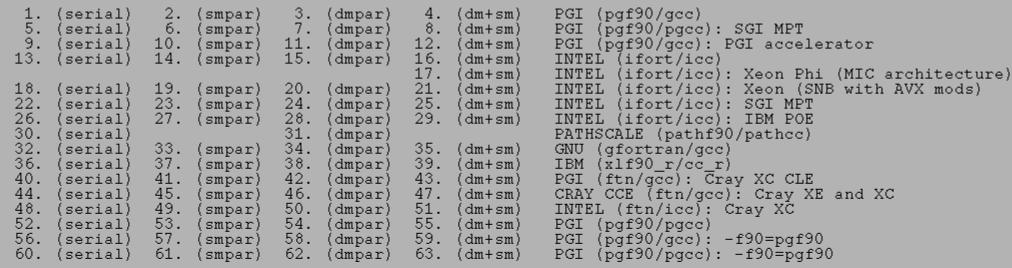
\includegraphics[width=0.85\textwidth]{linuxoptions.png}
    \caption{Opções computacionais disponíveis para seleção na compilação do COAWST.}
    \label{compskerana}
\end{figure}
\bigskip

\noindent Agora, no mesmo arquivo, procure pelas seguintes linhas:
\bigskip

\begin{bashcode}[fontsize=\footnotesize]
printf "Compile for nesting? (1=basic, 2=preset moves, 3=vortex following) [default 1]: " ;
}
$response = <STDIN> ;
\end{bashcode}
\bigskip

\noindent E modifique o \textit{<STDIN>} para o modo básico de aninhamento do modelo atmosférico WRF, como o exemplo a seguir:
\bigskip

\begin{bashcode}[fontsize=\footnotesize]
printf "Compile for nesting? (1=basic, 2=preset moves, 3=vortex following) [default 1]: " ;
}
$response = 1 ;
\end{bashcode}
\bigskip

\section{Compilando o MCT}
\bigskip

\begin{tcolorbox}[enhanced,
  grow to left by=0cm,%   equivalent to negative mdframed 'leftmargin'
  grow to right by=0cm,%  equivalent to negative mdframed 'rightmargin'
  enlarge top by=0cm,%     equivalent to mdframed 'skipabove'
  enlarge bottom by=0cm,%  equivalent to mdframed 'skipbelow'
  tcbox raise base,
  boxrule=1.0pt,
  left=18mm,
  colframe=red!50!black,coltext=red!25!black,colback=red!10!white,
  overlay={\begin{tcbclipinterior}\fill[red!75!blue!50!white] (frame.south west)
    rectangle node[text=white,font=\sffamily\bfseries\footnotesize,rotate=0] {ATENÇÃO} ([xshift=18mm]frame.north west);\end{tcbclipinterior}}]
Este guia utiliza o COAWST v 3.4.
\end{tcolorbox}
\bigskip


\noindent Deve-se compilar o MCT antes de compilar o COAWST. Neste caso, é necessário utilizar o arquivo \textit{setup\_pgi.sh}. Este arquivo foi copiado do repositório anterior, sendo indispensável alterar os diretórios contidos nele.
Portanto:
\bigskip

\begin{bashcode}
nedit setup_pgi.sh
\end{bashcode}
\bigskip

\noindent Caso necessário, altere os diretórios de acordo com o nome da sua pasta do COAWST e execute o arquivo para carregar os módulos necessários:
\bigskip

\begin{bashcode}
source setup_pgi.sh
\end{bashcode}
\bigskip

\noindent As bibliotecas serão ativadas, conforme apresentado na Figura \textcolor{bleu_cite}{\ref{modulos}}:
\bigskip


\begin{figure}[H]
    \centering
    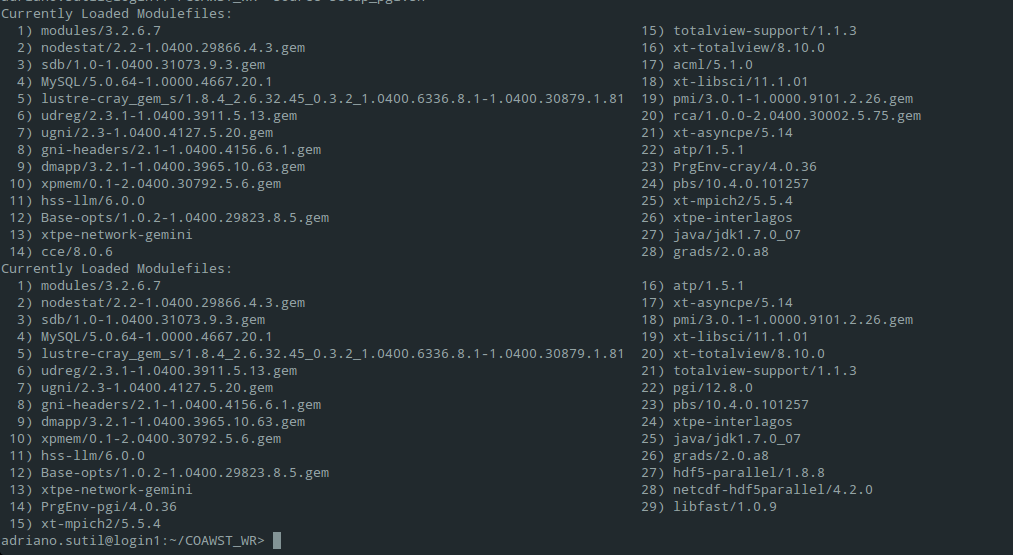
\includegraphics[width=0.85\textwidth]{modules.png}
    \caption{Módulos ativados no cluster com o arquivo \textit{setup\_pgi.sh} para o usuário adriano.sutil.}
    \label{modulos}
\end{figure}
\bigskip


\noindent Entre na pasta do MCT:
\bigskip

\begin{bashcode}
cd /home/nome.sobrenome/COAWST/Lib/MCT
\end{bashcode}
\bigskip

\noindent Abra o arquivo \textit{Makefile.conf}:
\bigskip


\begin{bashcode}
nedit Makefile.conf
\end{bashcode}
\bigskip

\noindent E modifique o arquivo conforme a seguir:
\bigskip

\begin{tcolorbox}[enhanced,
  grow to left by=0cm,%   equivalent to negative mdframed 'leftmargin'
  grow to right by=0cm,%  equivalent to negative mdframed 'rightmargin'
  enlarge top by=0cm,%     equivalent to mdframed 'skipabove'
  enlarge bottom by=0cm,%  equivalent to mdframed 'skipbelow'
  tcbox raise base,
  boxrule=1.0pt,
  left=18mm,
  colframe=red!50!black,coltext=red!25!black,colback=red!10!white,
  overlay={\begin{tcbclipinterior}\fill[red!75!blue!50!white] (frame.south west)
    rectangle node[text=white,font=\sffamily\bfseries\footnotesize,rotate=0] {ATENÇÃO} ([xshift=18mm]frame.north west);\end{tcbclipinterior}}]
Lembre-se de alterar o \textit{nome.sobrenome} dos diretórios!
\end{tcolorbox}
\bigskip

\begin{bashcode}
FC  	    = ftn
FCFLAGS	 = -O2
F90FLAGS        = 
REAL8           = -r8
ENDIAN          = -Mbyteswapio
INCFLAG         = -I
INCPATH         =
MPILIBS         = 
DEFS            = -DSYSLINUX -DCPRPGI
FPP	     = cpp
FPPFLAGS        = -P -C -N -traditional
CC              = cc
ALLCFLAGS       = -DFORTRAN_UNDERSCORE_ -DSYSLINUX -DCPRPGI -O
COMPILER_ROOT   = 
BABELROOT       = 
PYTHON          = 
PYTHONOPTS      = 
FORT_SIZE       = 
CRULE           = .c.o
90RULE          = .F90.o
F90RULECPP      = .F90RULECPP
INSTALL         = /home/nome.sobrenome/COAWST/Lib/MCT/install-sh -c
MKINSTALLDIRS   = /home/nome.sobrenome/COAWST/Lib/MCT/mkinstalldirs
abs_top_builddir= /home/nome.sobrenome/COAWST/Lib/MCT/
MCTPATH         = /home/nome.sobrenome/COAWST/Lib/MCT/mct
MPEUPATH        = /home/nome.sobrenome/COAWST/Lib/MCT/mpeu
EXAMPLEPATH     = /home/nome.sobrenome/COAWST/Lib/MCT/examples
MPISERPATH      = 
libdir          = /home/nome.sobrenome/COAWST/Lib/MCT/pgi/lib
includedir      = /home/nome.sobrenome/COAWST/Lib/MCT/pgi/include
AR	      = ar cq
RM	      = rm -f
\end{bashcode}
\bigskip

\noindent Instale o MCT digitando no terminal os seguintes comandos:
\bigskip

\begin{bashcode}
make
make install
\end{bashcode}
\bigskip
\noindent Observe as mensagens que aparecem no terminal e busque por erros. Caso negativo, o MCT foi compilado com sucesso.
\bigskip


\section{Compilando o caso-teste Sandy}
\bigskip

\noindent Existem dentro do COAWST alguns casos-teste para serem compilados e trabalhados. Neste caso compilaremos o projeto do furacão Sandy, que acopla e aninha o WRF, ROMS e SWAN. Primeiramente, é necessário conhecer a estrutura das pastas e arquivos do COAWST.
\bigskip

\noindent A estrutura típica de diretórios do COAWST está exemplificada na Figura \textcolor{bleu_cite}{\ref{pastascoa}}:
\bigskip

\begin{figure}[H]
    \centering
    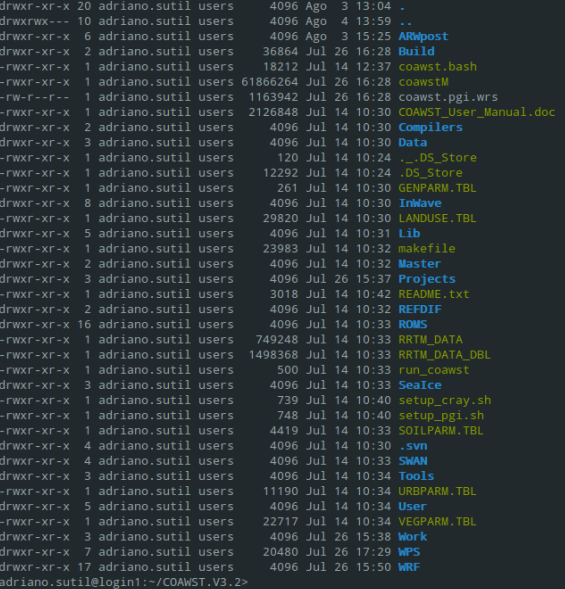
\includegraphics[width=0.50\textwidth]{estruturacoawst.png}
    \caption{Representação da pasta principal do COAWST e as subpastas.}
    \label{pastascoa}
\end{figure}
\bigskip

\noindent Serão utilizadas principalmente as pastas \textit{Projects} e \textit{Work}.

\subsection{Pasta Projects}\index{Pasta Projects}
\bigskip

\noindent Na pasta \textit{COAWST/Projects/Sandy} deverão constar os seguintes arquivos:
\bigskip

\begin{itemize}
\item Bound\_spec\_command
\item coastline.mat
\item coupling\_sandy.in
\item create\_sandy\_application.m
\item hycom\_info.mat
\item ijcoast.mat
\item multi\_1.at\_10m.dp.201210.grb2
\item multi\_1.at\_10m.hs.201210.grb2
\item multi\_1.at\_10m.tp.201210.grb2
\item namelist.input
\item ocean\_sandy.in
\item roms\_master\_climatology\_sandy.m
\item roms\_narr\_Oct2012.nc
\item roms\_narr\_ref3\_Oct2012.nc
\item Rweigths.txt
\item Sandy\_bdy.nc
\item Sandy\_clm.nc
\item Sandy\_clm\_ref3.nc
\item sandy.h
\item Sandy\_ini.nc
\item Sandy\_ini\_ref3.nc
\item Sandy\_init.hot
\item Sandy\_ref3\_init.hot
\item Sandy\_roms\_contact.nc
\item Sandy\_roms\_grid.nc
\item Sandy\_roms\_grid\_ref3.nc
\item Sandy\_swan\_bathy.bot
\item Sandy\_swan\_bathy\_ref3.bot
\item Sandy\_swan\_coord.grd
\item Sandy\_swan\_coord\_ref3.grd
\item scrip\_sandy\_moving.nc
\item scrip\_sandy\_static.nc
\item specpts.mat
\item swan\_narr\_Oct2012.dat
\item swan\_narr\_ref3\_Oct2012.dat
\item swan\_sandy.in
\item swan\_sandy\_ref3.in
\item tide\_forc\_Sandy.nc
\item TPAR10.txt
\item TPAR11.txt
\item TPAR12.txt
\item TPAR13.txt
\item TPAR14.txt
\item TPAR15.txt
\item TPAR16.txt
\item TPAR17.txt
\item TPAR18.txt
\item TPAR1.txt
\item TPAR2.txt
\item TPAR3.txt
\item TPAR4.txt
\item TPAR5.txt
\item TPAR6.txt
\item TPAR7.txt
\item TPAR8.txt
\item TPAR9.txt
\item USeast\_bathy.mat
\item Uweigths.txt
\item Vweigths.txt
\item wrfbdy\_d01
\item wrfinput\_d01
\item wrfinput\_d02
\item wrflowinp\_d01
\item wrflowinp\_d02
\end{itemize}
\bigskip

\subsection{Pasta Work}\index{Pasta Work}\label{workcoawstsec}
\bigskip

\noindent Para facilitar o gerenciamento das simulações, é sugerida a criação da pasta \textit{Work} no diretório principal do COAWST, com cada projeto inserido separadamente dentro dele. É nesta pasta que será simulado caso teste.
\bigskip

\begin{bashcode}
cd /scratch/nome.sobrenome/COAWST
mkdir Work
cd Work
mkdir Sandy
\end{bashcode}
\bigskip

\noindent Dentro da pasta \textit{/scratch/nome.sobrenome/COAWST/Work/Sandy} deverão conter os seguintes arquivos:
\bigskip

\begin{itemize}
\item run\_sandy.sh
\item limpa.sh
\item link.sh
\end{itemize}
\bigskip

\noindent O arquivo \textit{run\_sandy.sh} é usado para iniciar a simulação, \textit{link.sh} gera links simbólicos na pasta \textit{Work}, que serão utilizados pelos modelos, e o \textit{limpa.sh} é utilizado para limpar a pasta caso ocorra um erro e seja necessário iniciar uma nova integração. Os arquivos se encontram dentro da pasta \textit{/repositorio/work\_coawst}.
\bigskip

\noindent Portanto:

\bigskip

\begin{bashcode}
cd /scratch/nome.sobrenome/repositorio/work_coawst
cp limpa.sh link.sh run_sandy.sh /scratch/nome.sobrenome/COAWST/Work/Sandy
\end{bashcode}
\bigskip

\noindent Vá até o diretório \textit{/scratch/nome.sobrenome/COAWST/Work/Sandy} e abra o arquivo \textit{run\_sandy.sh}:
\bigskip

\begin{bashcode}
cd /scratch/nome.sobrenome/COAWST/Work/Sandy
nedit run_sandy.sh
\end{bashcode}
\bigskip

\noindent Procure os comandos a seguir e modifique os diretórios de acordo com o seu nome de usuário:
\bigskip

\begin{bashcode}
PBS -o /scratch/nome.sobrenome/COAWST/Work/Sandy/rws_total.out
ROOTDIR=/scratch/nome.sobrenome/COAWST
\end{bashcode}
\bigskip


\subsection{Compilando o caso teste}\index{Compilar o caso teste Sandy}
\bigskip

\noindent Vá para a pasta do projeto Sandy:
\bigskip

\begin{bashcode}
/home/nome.sobrenome/COAWST/Projects/Sandy
\end{bashcode}
\bigskip

\noindent Abra os seguintes arquivos para realizar modificações nos próximos passos:
\bigskip

\begin{itemize}
\item coupling\_sandy.in
\item swan\_sandy.in
\item swan\_sandy\_ref3.in
\item ocean\_sandy.in
\end{itemize}
\bigskip

\begin{bashcode}
nedit coupling_sandy.in swan_sandy.in swan_sandy_ref3.in ocean_sandy.in
\end{bashcode}
\bigskip

\noindent No arquivo \textit{coupling\_sandy.in} procure pela linha de comando abaixo e substitua:
\bigskip

\begin{bashcode}
OCN_name = Projects/Sandy/ocean_sandy.in
\end{bashcode}
\bigskip

\noindent Por:
\bigskip

\begin{bashcode}
OCN_name = /scratch/nome.sobrenome/COAWST/Projects/Sandy/ocean_sandy.in
\end{bashcode}
\bigskip

\noindent Nos arquivos \textit{swan\_sandy.in} e \textit{swan\_sandy\_ref3.in} complete todos os caminhos dos diretórios abaixo:
\bigskip

\noindent Modifique:
\bigskip

\begin{bashcode}
READGRID COORDINATES 1 'Projects/Sandy/Sandy_swan_coord.grd' 4 0 0 FREE
READINP BOTTOM 1 'Projects/Sandy/Sandy_swan_bathy.bot' 4 0 FREE
&READINP WIND 1 'Projects/Sandy/swan_namnarr_30Sep10Nov2012.dat' 4 0 FREE
INITIAL HOTSTART SINGLE 'Projects/Sandy/Sandy_init.hot'
\end{bashcode}
\bigskip

\noindent Por:
\bigskip

\begin{bashcode}[fontsize=\scriptsize]
READGRID COORDINATES 1 '/scratch/nome.sobrenome/COAWST/Projects/Sandy/Sandy_swan_coord.grd' 4 0 0 FREE
READINP BOTTOM 1 '/scratch/nome.sobrenome/COAWST/Projects/Sandy/Sandy_swan_bathy.bot' 4 0 FREE
&READINP WIND 1 '/scratch/nome.sobrenome/COAWST/Projects/Sandy/swan_namnarr_30Sep10Nov2012.dat' 4 0 FREE
INITIAL HOTSTART SINGLE '/scratch/nome.sobrenome/COAWST/Projects/Sandy/Sandy_init.hot'
\end{bashcode}
\bigskip

\noindent E no arquivo \textit{ocean\_sandy.in} procure pelas linhas de comando abaixo e substitua:
\bigskip

\begin{bashcode}
MyAppCPP = SANDY
VARNAME  = ROMS/External/varinfo.dat
GRDNAME == Projects/Sandy/Sandy_roms_grid.nc \
           Projects/Sandy/Sandy_roms_grid_ref3.nc
ININAME == Projects/Sandy/Sandy_ini.nc \
           Projects/Sandy/Sandy_ini_ref3.nc
NGCNAME =  Projects/Sandy/Sandy_roms_contact.nc
BRYNAME == Projects/Sandy/Sandy_bdy.nc
FRCNAME == Projects/Sandy/roms_narr_Oct2012.nc \
           Projects/Sandy/roms_narr_ref3_Oct2012.nc
\end{bashcode}
\bigskip

\noindent Por:
\bigskip

\begin{bashcode}[fontsize=\footnotesize]
MyAppCPP = Sandy
VARNAME  = /scratch/nome.sobrenome/COAWST/ROMS/External/varinfo.dat
GRDNAME == /scratch/nome.sobrenome/COAWST/Projects/Sandy/Sandy_roms_grid.nc \
           /scratch/nome.sobrenome/COAWST/Projects/Sandy/Sandy_roms_grid_ref3.nc
ININAME == /scratch/nome.sobrenome/COAWST/Projects/Sandy/Sandy_ini.nc \
           /scratch/nome.sobrenome/COAWST/Projects/Sandy/Sandy_ini_ref3.nc
NGCNAME =  /scratch/nome.sobrenome/COAWST/Projects/Sandy/Sandy_roms_contact.nc
BRYNAME == /scratch/nome.sobrenome/COAWST/Projects/Sandy/Sandy_bdy.nc
FRCNAME == /scratch/nome.sobrenome/COAWST/Projects/Sandy/roms_narr_Oct2012.nc \
           /scratch/nome.sobrenome/COAWST/Projects/Sandy/roms_narr_ref3_Oct2012.nc
\end{bashcode}
\bigskip

\noindent Volte para a pasta principal do COAWST e abra o arquivo \textit{coawst.bash}:
\bigskip

\begin{bashcode}
cd /scratch/nome.sobrenome/COAWST
nedit coawst.bash
\end{bashcode}
\bigskip

\noindent Procure os seguintes comandos e modifique, se necessário:
\bigskip

\begin{bashcode}
export   COAWST_APPLICATION=JOE_TC
export   MY_ROOT_DIR=${HOME}/COAWST
export   MY_HEADER_DIR=${MY_PROJECT_DIR}/Projects/JOE_TC
\end{bashcode}
\bigskip

\noindent Por:
\bigskip

\begin{bashcode}
export   COAWST_APPLICATION=Sandy
export   MY_ROOT_DIR=${HOME}/COAWST
export   MY_HEADER_DIR=${MY_PROJECT_DIR}/Projects/Sandy
\end{bashcode}
\bigskip

\noindent Ative novamente os módulos no arquivo \textit{setup\_pgi.sh}, e depois compile o projeto com o comando:
\bigskip

\begin{bashcode}
./coawst.bash -j 4  1> coawst.pgi.sandy 2>&1 &
\end{bashcode}
\bigskip

\noindent Este comando criará o arquivo de texto \textit{coawst.pgi.sandy} onde será possível acompanhar a evolução da compilação. Abra o arquivo de texto com o comando a seguir e procure pela mensagem final, como na Figura \textcolor{bleu_cite}{\ref{compcoafinal}}.
\bigskip

\begin{bashcode}
nedit coawst.pgi.sandy
\end{bashcode}
\bigskip

\begin{figure}[H]
    \centering
    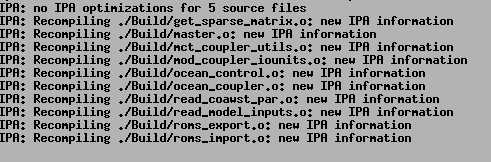
\includegraphics[width=0.65\textwidth]{coawstfinal.png}
    \caption{Mensagem final após compilar o COAWST.}
    \label{compcoafinal}
\end{figure}
\bigskip

\noindent Caso queira acompanhar pelo terminal a evolução da compilação, utilize o comando:
\bigskip

\begin{bashcode}
tail -f coawst.pgi.sandy
\end{bashcode}
\bigskip

\begin{tcolorbox}[enhanced,
  grow to left by=0cm,%   equivalent to negative mdframed 'leftmargin'
  grow to right by=0cm,%  equivalent to negative mdframed 'rightmargin'
  enlarge top by=0cm,%     equivalent to mdframed 'skipabove'
  enlarge bottom by=0cm,%  equivalent to mdframed 'skipbelow'
  tcbox raise base,
  boxrule=1.0pt,
  left=18mm,
  colframe=red!50!black,coltext=red!25!black,colback=red!10!white,
  overlay={\begin{tcbclipinterior}\fill[red!75!blue!50!white] (frame.south west)
    rectangle node[text=white,font=\sffamily\bfseries\footnotesize,rotate=0] {ATENÇÃO} ([xshift=18mm]frame.north west);\end{tcbclipinterior}}]
O processo de compilação é longo!
\end{tcolorbox}
\bigskip


\noindent Pronto! No diretório principal do COAWST, será criado um arquivo chamado \textit{coawstM}. Neste arquivo estarão compiladas todas as informações do seu projeto. Agora com o COAWST compilado, iniciaremos o caso teste.
\bigskip

\section{Simulando o caso teste Sandy}\label{sandyexec}
\bigskip

\noindent Para simular o caso, busque pela pasta \textit{Work/Sandy}. Digite:
\bigskip


\begin{bashcode}
cd /scratch/nome.sobrenome/COAWST/Work/Sandy
nedit run_sandy.sh
\end{bashcode}
\bigskip

\begin{tcolorbox}[enhanced,
  grow to left by=0cm,%   equivalent to negative mdframed 'leftmargin'
  grow to right by=0cm,%  equivalent to negative mdframed 'rightmargin'
  enlarge top by=0cm,%     equivalent to mdframed 'skipabove'
  enlarge bottom by=0cm,%  equivalent to mdframed 'skipbelow'
  tcbox raise base,
  boxrule=1.0pt,
  left=18mm,
  colframe=red!50!black,coltext=red!25!black,colback=red!10!white,
  overlay={\begin{tcbclipinterior}\fill[red!75!blue!50!white] (frame.south west)
    rectangle node[text=white,font=\sffamily\bfseries\footnotesize,rotate=0] {ATENÇÃO} ([xshift=18mm]frame.north west);\end{tcbclipinterior}}]
A pasta \textit{Work} deverá conter os arquivos \textit{limpa.sh}, \textit{link.sh} e \textit{run\_sandy.sh}. Eles poderão ser encontrados na pasta usada como repositório. Relembre a Seção \textcolor{bleu_cite}{\ref{workcoawstsec}}.
\end{tcolorbox}
\bigskip

\noindent Ao abrir o arquivo, verifique se os diretórios estão de acordo com o seu nome de usuário e digite o comando abaixo para iniciar a integração.
\bigskip

\begin{bashcode}
qsub run_sandy.sh
\end{bashcode}
\bigskip

\begin{tcolorbox}[enhanced,
  grow to left by=0cm,%   equivalent to negative mdframed 'leftmargin'
  grow to right by=0cm,%  equivalent to negative mdframed 'rightmargin'
  enlarge top by=0cm,%     equivalent to mdframed 'skipabove'
  enlarge bottom by=0cm,%  equivalent to mdframed 'skipbelow'
  tcbox raise base,
  boxrule=1.0pt,
  left=18mm,
  colframe=red!50!black,coltext=red!25!black,colback=red!10!white,
  overlay={\begin{tcbclipinterior}\fill[red!75!blue!50!white] (frame.south west)
    rectangle node[text=white,font=\sffamily\bfseries\footnotesize,rotate=0] {ATENÇÃO} ([xshift=18mm]frame.north west);\end{tcbclipinterior}}]
O comando \textit{qsub} submeterá o seu \textit{job}. Ele enviará o script executado para um lote do cluster, reservando uma parte dos processadores para a sua simulação.
\end{tcolorbox}
\bigskip

\noindent O processo gerará dois arquivos para acompanhar a evolução da simulação: o \textit{log.out} e \textit{log.err}. Para abrir, utilize:
\bigskip

\begin{bashcode}
nedit log.out log.err
\end{bashcode}
\bigskip

\noindent Ou acompanhe diretamente no terminal com o comando:
\bigskip

\begin{bashcode}
tail -f log.out
\end{bashcode}
\bigskip

\noindent As saídas das simulações serão armazenadas na pasta \textit{Work/Sandy}. Caso algum erro ocorra, limpe a área de trabalho com o comando:
\bigskip

\begin{bashcode}
./limpa.sh
\end{bashcode}
\bigskip


\begin{tcolorbox}[enhanced,
  grow to left by=0cm,%   equivalent to negative mdframed 'leftmargin'
  grow to right by=0cm,%  equivalent to negative mdframed 'rightmargin'
  enlarge top by=0cm,%     equivalent to mdframed 'skipabove'
  enlarge bottom by=0cm,%  equivalent to mdframed 'skipbelow'
  tcbox raise base,
  boxrule=1.0pt,
  left=18mm,
  colframe=red!50!black,coltext=red!25!black,colback=red!10!white,
  overlay={\begin{tcbclipinterior}\fill[red!75!blue!50!white] (frame.south west)
    rectangle node[text=white,font=\sffamily\bfseries\footnotesize,rotate=0] {ATENÇÃO} ([xshift=18mm]frame.north west);\end{tcbclipinterior}}]
A simulação do caso teste Sandy poderá demorar 5 horas ao integrar usando 3 processadores.
\end{tcolorbox}
\bigskip
